%\mychapter{6}{Results}

\section{Results}
%{Here are the results and what they mean! (3-4 days)}

\subsection{Simulation results }

% DF on noisy sim FR

%\begin{frame}[allowframebreaks]
%\begin{figure}
%\centering
%\begin{subfigure}{.5\textwidth}
%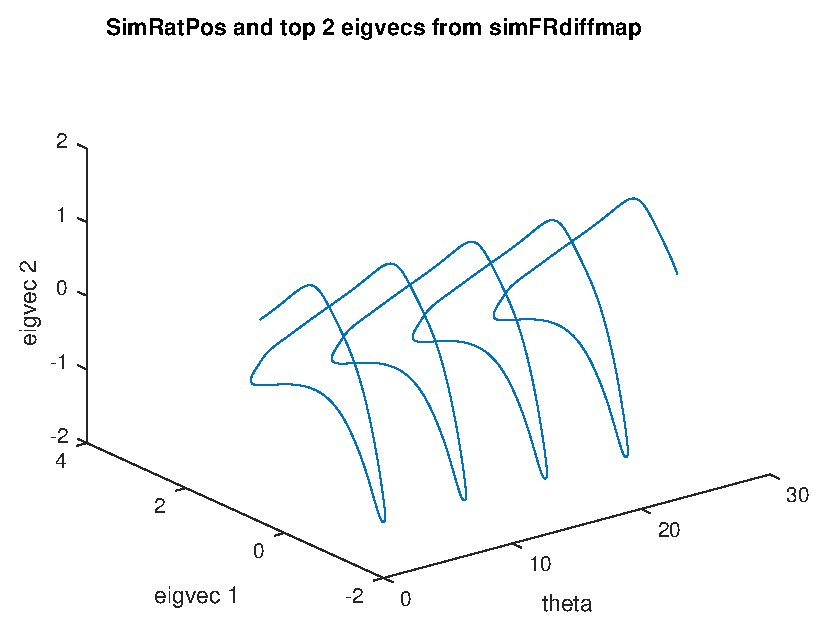
\includegraphics[page=1,width=\textwidth]{MI_on_SimNoisyFRdiffmap1.eps}
%\caption{DF on sim FR.}
%\end{subfigure}%
%\begin{subfigure}{0.5\textwidth}
%\includegraphics[page=2,width=\textwidth]{MI_on_SimNoisyFRdiffmap2.eps}
%\caption{DF on sim FR.}
%\end{subfigure}
%\end{figure}
%\end{frame}
%
%
%\vspace{2in}
%\begin{frame}[allowframebreaks]
%\begin{figure}
%\centering
%\begin{subfigure}{.5\textwidth}
%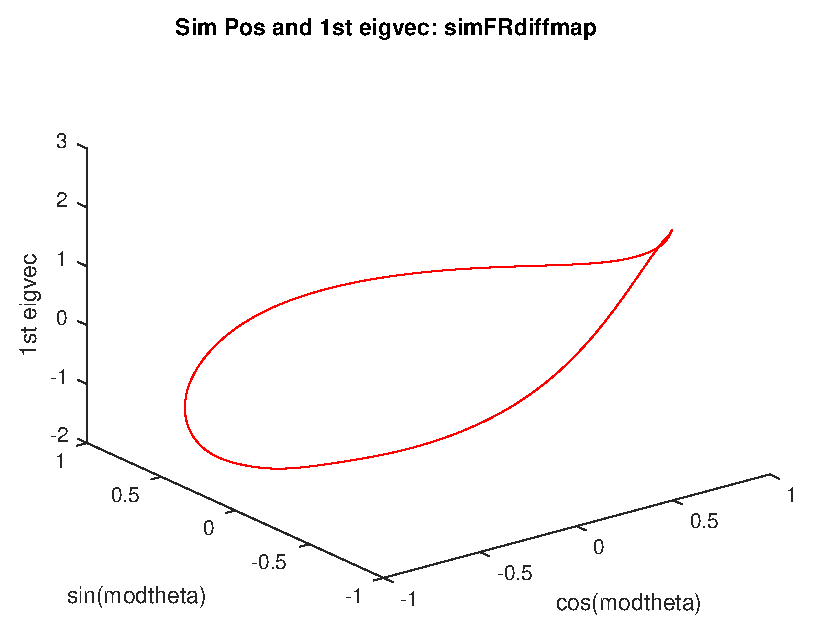
\includegraphics[page=1,width=\textwidth]{MI_on_SimNoisyFRdiffmap3.eps}
%\caption{DF on sim FR.}
%\end{subfigure}%
%\begin{subfigure}{0.5\textwidth}
%\includegraphics[page=2,width=\textwidth]{MI_on_SimNoisyFRdiffmap4.eps}
%\caption{DF on sim FR.}
%\end{subfigure}
%\end{figure}
%\end{frame}
%
%
%
%
%
%
%
%
%



\subsection{Results on Real-world  Data}
\begin{frame}[allowframebreaks]
\begin{figure}
\centering
\begin{subfigure}{.5\textwidth}
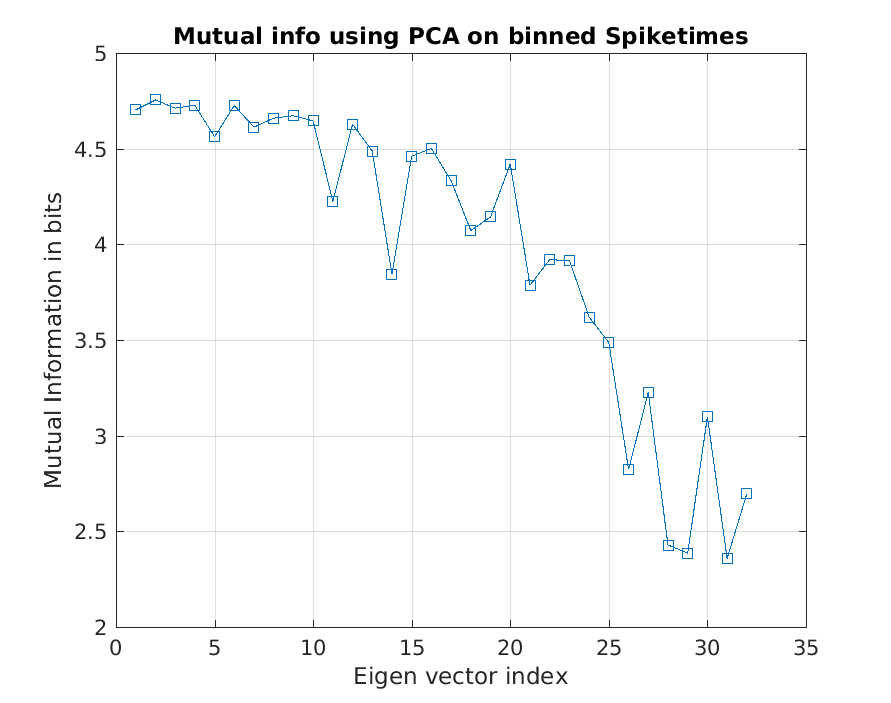
\includegraphics[page=1,width=\textwidth]{MI_binpca_real.png}
\caption{PCA on binnedSpikes.}
\end{subfigure}%
\begin{subfigure}{0.5\textwidth}
\includegraphics[page=2,width=\textwidth]{MI_bindiffMaps_real.png}
\caption{DF on binnedSpikes.}
\end{subfigure}
\end{figure}
\end{frame}


\vspace{2in}
\begin{frame}[allowframebreaks]
\begin{figure}
\centering
\begin{subfigure}{.5\textwidth}
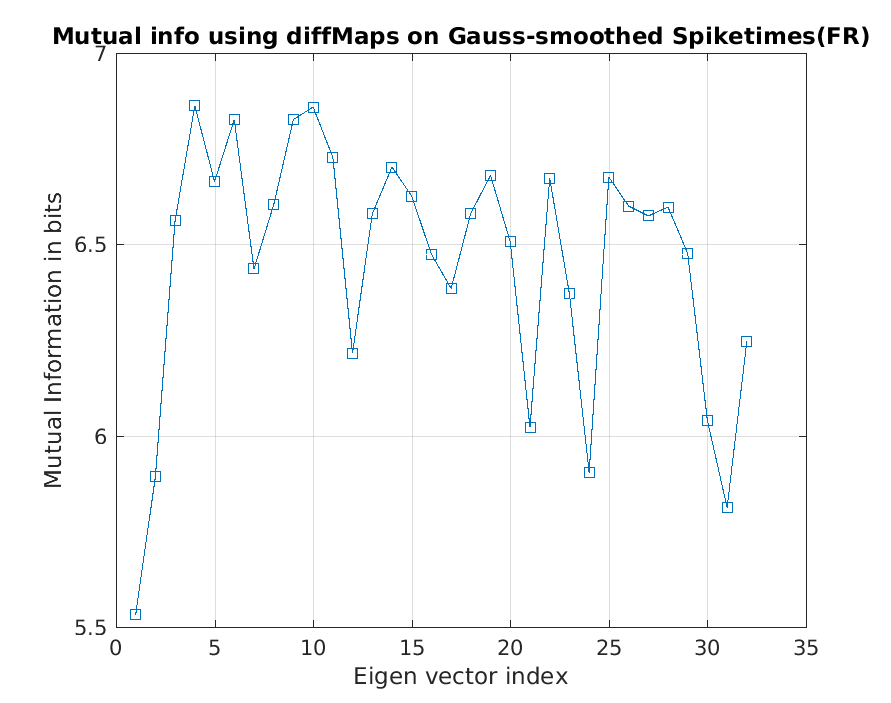
\includegraphics[page=1,width=\textwidth]{MI_FRdiffMaps_real.png}
\caption{DF on smoothedSpikes.}
\end{subfigure}%
\begin{subfigure}{0.5\textwidth}
\includegraphics[page=2,width=\textwidth]{MI_FRpca_real.png}
\caption{PCA on smoothedSpikes.}
\end{subfigure}
\end{figure}
\end{frame}


\vspace{1in}
\begin{frame}[allowframebreaks]
\begin{figure}
\centering
\begin{subfigure}{.5\textwidth}
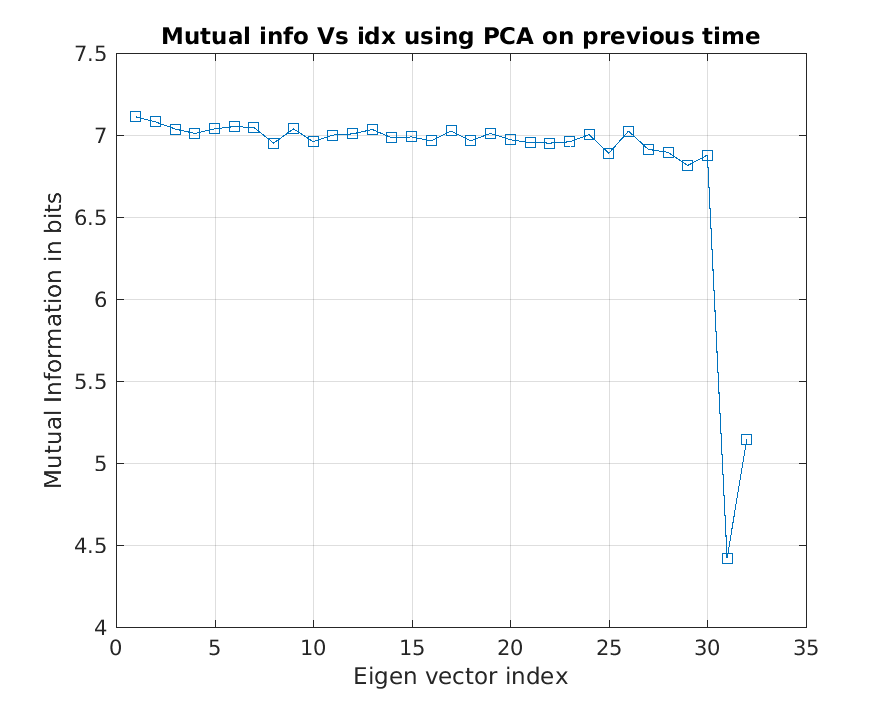
\includegraphics[page=1,width=\textwidth]{MI_PCA_prevtime_real.png}
\caption{PCA on prevtime.}
\end{subfigure}%
\begin{subfigure}{0.5\textwidth}
\includegraphics[page=2,width=\textwidth]{MI_prevDiffMaps_real.png}
\caption{DF on prevtime.}
\end{subfigure}
\end{figure}
\end{frame}









\newpage





















%\begin{itemize}
%\item show the graphs/results package
%\item this is how we're interpreting the results
%\item why does this matter?
%\item what measure of goodness did you use?
%(Fisher Vs Shannon information)

%%==========suggested by Duane============================================
%\item Mention that there are other ways of checking measures of goodness
% e.g the one provided by diffusion maps, Bayesian decoding refer to the nature
% and review artcicle.


%\end{itemize}







